\begin{tikzpicture}[scale=.2, anchor=base]
\node[draw=black] (sn0x9b931a0W9) at (9, -10) {\begin{tikzpicture}[scale=.2]
\node[circle, scale=0.75, fill] (tid0) at (0,0){};
\node[circle, scale=0.75, fill] (tid1) at (0,1.5){};
\node[circle, scale=0.75, fill, red] (tid4) at (0,3){};

\draw[](tid1) -- (tid4);

\node[circle, scale=0.75, fill] (tid2) at (1.5,1.5){};
\node[circle, scale=0.75, fill] (tid5) at (1.5,3){};

\draw[](tid2) -- (tid5);

\node[circle, scale=0.75, fill] (tid3) at (3,1.5){};
\node[circle, scale=0.75, fill, red] (tid6) at (3,3){};

\draw[](tid3) -- (tid6);

\draw[](tid0) -- (tid1);
\draw[](tid0) -- (tid2);
\draw[](tid0) -- (tid3);

\end{tikzpicture}
};
\node[draw=black] (sn0x9b93f30W9) at (9, -20) {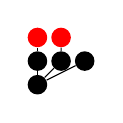
\begin{tikzpicture}[scale=.2]
\node[circle, scale=0.75, fill] (tid0) at (0,0){};
\node[circle, scale=0.75, fill] (tid1) at (0,1.5){};
\node[circle, scale=0.75, fill, red] (tid4) at (0,3){};

\draw[](tid1) -- (tid4);

\node[circle, scale=0.75, fill] (tid2) at (1.5,1.5){};
\node[circle, scale=0.75, fill, red] (tid5) at (1.5,3){};

\draw[](tid2) -- (tid5);

\node[circle, scale=0.75, fill] (tid3) at (3,1.5){};

\draw[](tid0) -- (tid1);
\draw[](tid0) -- (tid2);
\draw[](tid0) -- (tid3);

\end{tikzpicture}
};
\node[draw=black] (sn0x9b94568W9) at (9, -30) {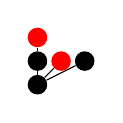
\begin{tikzpicture}[scale=.2]
\node[circle, scale=0.75, fill] (tid0) at (0,0){};
\node[circle, scale=0.75, fill] (tid1) at (0,1.5){};
\node[circle, scale=0.75, fill, red] (tid4) at (0,3){};

\draw[](tid1) -- (tid4);

\node[circle, scale=0.75, fill, red] (tid2) at (1.5,1.5){};

\node[circle, scale=0.75, fill] (tid3) at (3,1.5){};

\draw[](tid0) -- (tid1);
\draw[](tid0) -- (tid2);
\draw[](tid0) -- (tid3);

\end{tikzpicture}
};
\node[draw=black] (sn0x9b94720W9) at (9, -40) {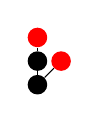
\begin{tikzpicture}[scale=.2]
\node[circle, scale=0.75, fill] (tid0) at (0,0){};
\node[circle, scale=0.75, fill] (tid1) at (0,1.5){};
\node[circle, scale=0.75, fill, red] (tid3) at (0,3){};

\draw[](tid1) -- (tid3);

\node[circle, scale=0.75, fill, red] (tid2) at (1.5,1.5){};

\draw[](tid0) -- (tid1);
\draw[](tid0) -- (tid2);

\end{tikzpicture}
};
\node[draw=black] (sn0x9b94990W9) at (9, -50) {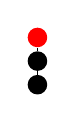
\begin{tikzpicture}[scale=.2]
\node[circle, scale=0.75, fill] (tid0) at (0,0){};
\node[circle, scale=0.75, fill] (tid1) at (0,1.5){};
\node[circle, scale=0.75, fill, red] (tid2) at (0,3){};

\draw[](tid1) -- (tid2);

\draw[](tid0) -- (tid1);

\end{tikzpicture}
};
\node[draw=black] (sn0x9b94cb0W9) at (9, -60) {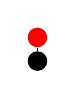
\begin{tikzpicture}[scale=.2]
\node[circle, scale=0.75, fill] (tid0) at (0,0){};
\node[circle, scale=0.75, fill, red] (tid1) at (0,1.5){};

\draw[](tid0) -- (tid1);

\end{tikzpicture}
};
\node[draw=black] (sn0x9b94d18W9) at (9, -70) {
\begin{tikzpicture}[scale=.2]
\node[circle, scale=0.75, fill] (tid0) at (0,0){};

\end{tikzpicture}
};
\draw (sn0x9b94cb0W9.south) -- (sn0x9b94d18W9.north);
\draw (sn0x9b94990W9.south) -- (sn0x9b94cb0W9.north);
\node[draw=black] (sn0x9b94b90W18) at (18, -50) {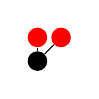
\begin{tikzpicture}[scale=.2]
\node[circle, scale=0.75, fill] (tid0) at (0,0){};
\node[circle, scale=0.75, fill, red] (tid1) at (0,1.5){};

\node[circle, scale=0.75, fill, red] (tid2) at (1.5,1.5){};

\draw[](tid0) -- (tid1);
\draw[](tid0) -- (tid2);

\end{tikzpicture}
};
\draw (sn0x9b94b90W18.south) -- (sn0x9b94cb0W9.north);
\draw (sn0x9b94720W9.south) -- (sn0x9b94990W9.north);
\draw (sn0x9b94720W9.south) -- (sn0x9b94b90W18.north);
\node[draw=black] (sn0x9b94788W18) at (18, -40) {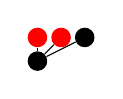
\begin{tikzpicture}[scale=.2]
\node[circle, scale=0.75, fill] (tid0) at (0,0){};
\node[circle, scale=0.75, fill, red] (tid1) at (0,1.5){};

\node[circle, scale=0.75, fill, red] (tid2) at (1.5,1.5){};

\node[circle, scale=0.75, fill] (tid3) at (3,1.5){};

\draw[](tid0) -- (tid1);
\draw[](tid0) -- (tid2);
\draw[](tid0) -- (tid3);

\end{tikzpicture}
};
\draw (sn0x9b94788W18.south) -- (sn0x9b94b90W18.north);
\draw (sn0x9b94568W9.south) -- (sn0x9b94720W9.north);
\draw (sn0x9b94568W9.south) -- (sn0x9b94788W18.north);
\draw (sn0x9b93f30W9.south) -- (sn0x9b94568W9.north);
\draw (sn0x9b931a0W9.south) -- (sn0x9b93f30W9.north);
\end{tikzpicture}

%%% Local Variables:
%%% TeX-master: "thesis/thesis.tex"
%%% End: 

\begin{tikzpicture}[scale=.2, anchor=base]
\node[draw=black] (sn0x9b93200W9) at (9, -10) {\begin{tikzpicture}[scale=.2]
\node[circle, scale=0.75, fill] (tid0) at (0,0){};
\node[circle, scale=0.75, fill] (tid1) at (0,1.5){};
\node[circle, scale=0.75, fill] (tid4) at (0,3){};

\draw[](tid1) -- (tid4);

\node[circle, scale=0.75, fill] (tid2) at (1.5,1.5){};
\node[circle, scale=0.75, fill, red] (tid5) at (1.5,3){};

\draw[](tid2) -- (tid5);

\node[circle, scale=0.75, fill] (tid3) at (3,1.5){};
\node[circle, scale=0.75, fill, red] (tid6) at (3,3){};

\draw[](tid3) -- (tid6);

\draw[](tid0) -- (tid1);
\draw[](tid0) -- (tid2);
\draw[](tid0) -- (tid3);

\end{tikzpicture}
};
\node[draw=black] (sn0x9b93f30W9) at (9, -20) {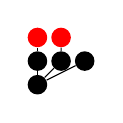
\begin{tikzpicture}[scale=.2]
\node[circle, scale=0.75, fill] (tid0) at (0,0){};
\node[circle, scale=0.75, fill] (tid1) at (0,1.5){};
\node[circle, scale=0.75, fill, red] (tid4) at (0,3){};

\draw[](tid1) -- (tid4);

\node[circle, scale=0.75, fill] (tid2) at (1.5,1.5){};
\node[circle, scale=0.75, fill, red] (tid5) at (1.5,3){};

\draw[](tid2) -- (tid5);

\node[circle, scale=0.75, fill] (tid3) at (3,1.5){};

\draw[](tid0) -- (tid1);
\draw[](tid0) -- (tid2);
\draw[](tid0) -- (tid3);

\end{tikzpicture}
};
\node[draw=black] (sn0x9b94568W9) at (9, -30) {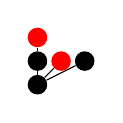
\begin{tikzpicture}[scale=.2]
\node[circle, scale=0.75, fill] (tid0) at (0,0){};
\node[circle, scale=0.75, fill] (tid1) at (0,1.5){};
\node[circle, scale=0.75, fill, red] (tid4) at (0,3){};

\draw[](tid1) -- (tid4);

\node[circle, scale=0.75, fill, red] (tid2) at (1.5,1.5){};

\node[circle, scale=0.75, fill] (tid3) at (3,1.5){};

\draw[](tid0) -- (tid1);
\draw[](tid0) -- (tid2);
\draw[](tid0) -- (tid3);

\end{tikzpicture}
};
\node[draw=black] (sn0x9b94720W9) at (9, -40) {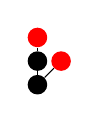
\begin{tikzpicture}[scale=.2]
\node[circle, scale=0.75, fill] (tid0) at (0,0){};
\node[circle, scale=0.75, fill] (tid1) at (0,1.5){};
\node[circle, scale=0.75, fill, red] (tid3) at (0,3){};

\draw[](tid1) -- (tid3);

\node[circle, scale=0.75, fill, red] (tid2) at (1.5,1.5){};

\draw[](tid0) -- (tid1);
\draw[](tid0) -- (tid2);

\end{tikzpicture}
};
\node[draw=black] (sn0x9b94990W9) at (9, -50) {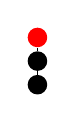
\begin{tikzpicture}[scale=.2]
\node[circle, scale=0.75, fill] (tid0) at (0,0){};
\node[circle, scale=0.75, fill] (tid1) at (0,1.5){};
\node[circle, scale=0.75, fill, red] (tid2) at (0,3){};

\draw[](tid1) -- (tid2);

\draw[](tid0) -- (tid1);

\end{tikzpicture}
};
\node[draw=black] (sn0x9b94cb0W9) at (9, -60) {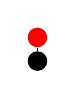
\begin{tikzpicture}[scale=.2]
\node[circle, scale=0.75, fill] (tid0) at (0,0){};
\node[circle, scale=0.75, fill, red] (tid1) at (0,1.5){};

\draw[](tid0) -- (tid1);

\end{tikzpicture}
};
\node[draw=black] (sn0x9b94d18W9) at (9, -70) {
\begin{tikzpicture}[scale=.2]
\node[circle, scale=0.75, fill] (tid0) at (0,0){};

\end{tikzpicture}
};
\draw (sn0x9b94cb0W9.south) -- (sn0x9b94d18W9.north);
\draw (sn0x9b94990W9.south) -- (sn0x9b94cb0W9.north);
\node[draw=black] (sn0x9b94b90W18) at (18, -50) {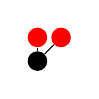
\begin{tikzpicture}[scale=.2]
\node[circle, scale=0.75, fill] (tid0) at (0,0){};
\node[circle, scale=0.75, fill, red] (tid1) at (0,1.5){};

\node[circle, scale=0.75, fill, red] (tid2) at (1.5,1.5){};

\draw[](tid0) -- (tid1);
\draw[](tid0) -- (tid2);

\end{tikzpicture}
};
\draw (sn0x9b94b90W18.south) -- (sn0x9b94cb0W9.north);
\draw (sn0x9b94720W9.south) -- (sn0x9b94990W9.north);
\draw (sn0x9b94720W9.south) -- (sn0x9b94b90W18.north);
\node[draw=black] (sn0x9b94788W18) at (18, -40) {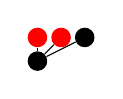
\begin{tikzpicture}[scale=.2]
\node[circle, scale=0.75, fill] (tid0) at (0,0){};
\node[circle, scale=0.75, fill, red] (tid1) at (0,1.5){};

\node[circle, scale=0.75, fill, red] (tid2) at (1.5,1.5){};

\node[circle, scale=0.75, fill] (tid3) at (3,1.5){};

\draw[](tid0) -- (tid1);
\draw[](tid0) -- (tid2);
\draw[](tid0) -- (tid3);

\end{tikzpicture}
};
\draw (sn0x9b94788W18.south) -- (sn0x9b94b90W18.north);
\draw (sn0x9b94568W9.south) -- (sn0x9b94720W9.north);
\draw (sn0x9b94568W9.south) -- (sn0x9b94788W18.north);
\draw (sn0x9b93f30W9.south) -- (sn0x9b94568W9.north);
\draw (sn0x9b93200W9.south) -- (sn0x9b93f30W9.north);
\end{tikzpicture}

%%% Local Variables:
%%% TeX-master: "thesis/thesis.tex"
%%% End: 

\begin{tikzpicture}[scale=.2, anchor=base]
\node[draw=black] (sn0x9b93260W9) at (9, -10) {\begin{tikzpicture}[scale=.2]
\node[circle, scale=0.75, fill] (tid0) at (0,0){};
\node[circle, scale=0.75, fill] (tid1) at (0,1.5){};
\node[circle, scale=0.75, fill, red] (tid4) at (0,3){};

\draw[](tid1) -- (tid4);

\node[circle, scale=0.75, fill] (tid2) at (1.5,1.5){};
\node[circle, scale=0.75, fill, red] (tid5) at (1.5,3){};

\draw[](tid2) -- (tid5);

\node[circle, scale=0.75, fill] (tid3) at (3,1.5){};
\node[circle, scale=0.75, fill] (tid6) at (3,3){};

\draw[](tid3) -- (tid6);

\draw[](tid0) -- (tid1);
\draw[](tid0) -- (tid2);
\draw[](tid0) -- (tid3);

\end{tikzpicture}
};
\node[draw=black] (sn0x9b93f30W9) at (9, -20) {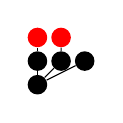
\begin{tikzpicture}[scale=.2]
\node[circle, scale=0.75, fill] (tid0) at (0,0){};
\node[circle, scale=0.75, fill] (tid1) at (0,1.5){};
\node[circle, scale=0.75, fill, red] (tid4) at (0,3){};

\draw[](tid1) -- (tid4);

\node[circle, scale=0.75, fill] (tid2) at (1.5,1.5){};
\node[circle, scale=0.75, fill, red] (tid5) at (1.5,3){};

\draw[](tid2) -- (tid5);

\node[circle, scale=0.75, fill] (tid3) at (3,1.5){};

\draw[](tid0) -- (tid1);
\draw[](tid0) -- (tid2);
\draw[](tid0) -- (tid3);

\end{tikzpicture}
};
\node[draw=black] (sn0x9b94568W9) at (9, -30) {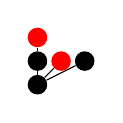
\begin{tikzpicture}[scale=.2]
\node[circle, scale=0.75, fill] (tid0) at (0,0){};
\node[circle, scale=0.75, fill] (tid1) at (0,1.5){};
\node[circle, scale=0.75, fill, red] (tid4) at (0,3){};

\draw[](tid1) -- (tid4);

\node[circle, scale=0.75, fill, red] (tid2) at (1.5,1.5){};

\node[circle, scale=0.75, fill] (tid3) at (3,1.5){};

\draw[](tid0) -- (tid1);
\draw[](tid0) -- (tid2);
\draw[](tid0) -- (tid3);

\end{tikzpicture}
};
\node[draw=black] (sn0x9b94720W9) at (9, -40) {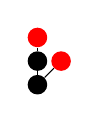
\begin{tikzpicture}[scale=.2]
\node[circle, scale=0.75, fill] (tid0) at (0,0){};
\node[circle, scale=0.75, fill] (tid1) at (0,1.5){};
\node[circle, scale=0.75, fill, red] (tid3) at (0,3){};

\draw[](tid1) -- (tid3);

\node[circle, scale=0.75, fill, red] (tid2) at (1.5,1.5){};

\draw[](tid0) -- (tid1);
\draw[](tid0) -- (tid2);

\end{tikzpicture}
};
\node[draw=black] (sn0x9b94990W9) at (9, -50) {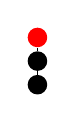
\begin{tikzpicture}[scale=.2]
\node[circle, scale=0.75, fill] (tid0) at (0,0){};
\node[circle, scale=0.75, fill] (tid1) at (0,1.5){};
\node[circle, scale=0.75, fill, red] (tid2) at (0,3){};

\draw[](tid1) -- (tid2);

\draw[](tid0) -- (tid1);

\end{tikzpicture}
};
\node[draw=black] (sn0x9b94cb0W9) at (9, -60) {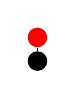
\begin{tikzpicture}[scale=.2]
\node[circle, scale=0.75, fill] (tid0) at (0,0){};
\node[circle, scale=0.75, fill, red] (tid1) at (0,1.5){};

\draw[](tid0) -- (tid1);

\end{tikzpicture}
};
\node[draw=black] (sn0x9b94d18W9) at (9, -70) {
\begin{tikzpicture}[scale=.2]
\node[circle, scale=0.75, fill] (tid0) at (0,0){};

\end{tikzpicture}
};
\draw (sn0x9b94cb0W9.south) -- (sn0x9b94d18W9.north);
\draw (sn0x9b94990W9.south) -- (sn0x9b94cb0W9.north);
\node[draw=black] (sn0x9b94b90W18) at (18, -50) {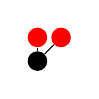
\begin{tikzpicture}[scale=.2]
\node[circle, scale=0.75, fill] (tid0) at (0,0){};
\node[circle, scale=0.75, fill, red] (tid1) at (0,1.5){};

\node[circle, scale=0.75, fill, red] (tid2) at (1.5,1.5){};

\draw[](tid0) -- (tid1);
\draw[](tid0) -- (tid2);

\end{tikzpicture}
};
\draw (sn0x9b94b90W18.south) -- (sn0x9b94cb0W9.north);
\draw (sn0x9b94720W9.south) -- (sn0x9b94990W9.north);
\draw (sn0x9b94720W9.south) -- (sn0x9b94b90W18.north);
\node[draw=black] (sn0x9b94788W18) at (18, -40) {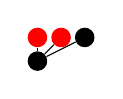
\begin{tikzpicture}[scale=.2]
\node[circle, scale=0.75, fill] (tid0) at (0,0){};
\node[circle, scale=0.75, fill, red] (tid1) at (0,1.5){};

\node[circle, scale=0.75, fill, red] (tid2) at (1.5,1.5){};

\node[circle, scale=0.75, fill] (tid3) at (3,1.5){};

\draw[](tid0) -- (tid1);
\draw[](tid0) -- (tid2);
\draw[](tid0) -- (tid3);

\end{tikzpicture}
};
\draw (sn0x9b94788W18.south) -- (sn0x9b94b90W18.north);
\draw (sn0x9b94568W9.south) -- (sn0x9b94720W9.north);
\draw (sn0x9b94568W9.south) -- (sn0x9b94788W18.north);
\draw (sn0x9b93f30W9.south) -- (sn0x9b94568W9.north);
\draw (sn0x9b93260W9.south) -- (sn0x9b93f30W9.north);
\end{tikzpicture}

%%% Local Variables:
%%% TeX-master: "thesis/thesis.tex"
%%% End: 

